86. \begin{figure}[ht!]
\center{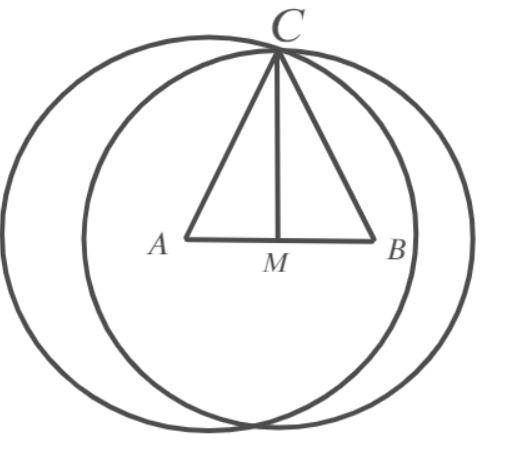
\includegraphics[scale=0.35]{g86.png}}
\end{figure}\\
Пусть $AB$ --- данная меньшая сторона. С помощью циркуля и линейки найдём её середину $M$ (это стандартное построение). После этого проведём две окружности: с радиусом, равным второй стороне и центром в точке $A$ и с радиусом, равным медиане и центром в точке $M.$ Пусть они пересекутся в точке $C$ (если такой точки нет, то соответствующего треугольника не существует). Тогда треугольник $ABC$ --- искомый.\\
